\chapter[SCP-131 “眼豆”]{
    SCP-131 The "Eye Pods"\\
    SCP-131 “眼豆”
}

\label{chap:SCP-131}

\begin{figure}[H]
    \centering
    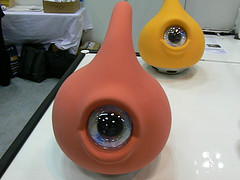
\includegraphics[width=0.5\linewidth]{images/SCP.131.jpg}
    \caption*{SCP-131-A 和 SCP-131-B}
\end{figure}

\bb{项目编号:}SCP-131

\bb{项目等级:}Safe

\bb{特殊收容措施:}SCP-131-A以及SCP-131-B不需要特殊的安全遏制程序,他们可以自由在Site19活动如此之久就像他们从未打算过进入任何禁区或者离开设施一样。对物体的非正式交流是被允许的,但建议此类交流应该最低限度地避免生物对有关人员产生依附。任何时间都将保持给此物体打上每小时一次的标签,但仍然不能解释这些时候他们的存在构成了一个一级封锁状态的原因。任何对此物体有虐待或辱骂的报告将会被严重处罚。

\bb{描述:}SCP-131-A和SCP-131-B(保安人员给他们取了个亲切的绰号“眼豆”)是一对眼泪状的生物,大概高30cm(1英尺),在他们身体的中间有一只独立的蓝眼,SCP-131-A是火橙色的,而SCP-131-B是深黄色。在这生物的底部是一个轮状突出物,这使他们能够运动,这或许意味着他们可能是生物的起源。这生物能够移动得令人惊奇地块,几乎能够在一秒内移动60米。然而,这生物缺乏制动(刹车)系统,这会导致一些壮观的情景,如果太兴奋,灾难就会降临到这些生物头上。这生物也展示了它们能够攀爬陡峭平面的能力,并且它们已经不止一次在通风口迷路了。

这些生物看上去拥有普通家猫的智商,并且拥有无法满足的好奇心。他们将大部分时间花在普通地在设施游荡中,并且观察工作中的SCP保安人员,还经常偷窥其他Safe级别的SCP物体。这些生物看上去可以通过某种无法测量的高频声互相交流。观察人员从未看见过他们眨眼,即使是将他们放在实验室被用录像观察18小时以上。

这些生物看上去很够很好地回应各种情绪,他们会很快地接近情绪的发出者并表达自己的情绪,他们接近的方式对一只幼犬和一个人是完全一样的。只要接触过,他们会跟随到底,即使是正常级限制区域。虽然好奇心旺盛,但是他们仍然能感知到附近的危险,而且,如果他们跟随的对象开始接近SCP-131们认为是危险的东西(比如Euclid和Keter级别的物体),他们会在对象脚旁不断蠕动(或者会适度地更激动)并用恐慌的音调发出咿呀声,就像警告他们一样。因为Site-19员工在处理Euclid或Keter级别的物体时经常会遇到危险,所以建议工作人员尽量避免被SCP-131们跟随,而且在一些细微的操作或实验期间他们(SCP-131)会心烦意乱,有可能给他们自身带来危险(详见附录 131-1)。如果被他们所跟随的人无视他们足够长的时间,他们经常会失去兴趣并回到正常的活动中去。

应该被记录的一点是,工作人员并不需要真挚的维护或关心他们,他们不吃不喝不排泄,甚至不睡觉,看上去他们需要的食物仅仅是视觉刺激(即使这种需求也需要进一步查证)。

SCP-131-A和SCP-131-B是在19██年,在████████████外的一个玉米田被发现的,他们迅速地经由{[}资料删除]被运到Site-19,并马上被降级为安全级别,当确认他们的消息没有外泄到任何敌对国外势力时,他们得到在Site的自由管理。

\bb{附录 131-1:}在 ████年\slash ██月\slash ██日 发生的事件,期间SCP-131们跟随这其中一名清洁员工,当时那名员工正在进行\hyperref[chap:SCP-173]{SCP-173}的放置设施的日常清洁。当SCP-131们尝试发出对该员工的危险警告被无视后,出于责任感,他们比该员工以及另外两名保安人员先一步冲进了SCP-173的放置设施。一进入到里面,员工们发现到他们正坐SCP-173前并在专心地看着它。就像在提醒他们SCP-173只有在看不到情况下才会移动一样。但清洁员工仍无视了该物体的存在并继续了两星期一次的常规清洁。当清洁队离开时,SCP-131们也同样离开了,他们背靠着出口缓慢离开,而且由始至终都看着SCP-173。最近将SCP-131-A及SCP-131-B作为对SCP-173(或其他需要持续注视的SCP,比如\hyperref[chap:SCP-689]{SCP-689})的“守望者”的应用计划正在考虑中。
